\documentclass[12pt]{article}

% a template that a friend gave, it's worked well enough for me
% i have added some packages and stuff that have proved useful

\usepackage{fancyhdr}
\usepackage{tipa}
\usepackage{fontspec}
\usepackage{amsfonts}
\usepackage{enumitem}
\usepackage[margin=1in]{geometry}
\usepackage{graphicx}
\usepackage{float}
\usepackage{amsmath}
\usepackage{braket}
\usepackage{amssymb}
\usepackage{booktabs}
\usepackage{hyperref}
\usepackage{mathtools}
\usepackage{xcolor}
\usepackage{float}
\usepackage{algpseudocodex}
\usepackage{titlesec}
\usepackage{bbm}

\pagestyle{fancy}
\fancyhf{} % sets both header and footer to nothing
\lhead{Kevin Sheng}
\setmainfont{Comic Neue}
\renewcommand{\headrulewidth}{1pt}
\setlength{\headheight}{0.75in}
\setlength{\oddsidemargin}{0in}
\setlength{\evensidemargin}{0in}
\setlength{\voffset}{-.5in}
\setlength{\headsep}{10pt}
\setlength{\textwidth}{6.5in}
\setlength{\headwidth}{6.5in}
\setlength{\textheight}{8in}
\renewcommand{\headrulewidth}{0.5pt}
\renewcommand{\footrulewidth}{0.3pt}
\setlength{\textwidth}{6.5in}
\usepackage{setspace}
\usepackage{multicol}
\usepackage{float}
\setlength{\columnsep}{1cm}
\setlength\parindent{24pt}
\usepackage [english]{babel}
\usepackage [autostyle, english = american]{csquotes}
\MakeOuterQuote{"}

\setlength{\parskip}{6pt}
\setlength{\parindent}{0pt}

\titlespacing\section{0pt}{12pt plus 4pt minus 2pt}{0pt plus 2pt minus 2pt}
\titlespacing\subsection{0pt}{12pt plus 4pt minus 2pt}{0pt plus 2pt minus 2pt}
\titlespacing\subsubsection{0pt}{12pt plus 4pt minus 2pt}{0pt plus 2pt minus 2pt}

\hypersetup{colorlinks=true, urlcolor=blue}

\newcommand{\correction}[1]{\textcolor{red}{#1}}


\rhead{ECE C147}

\DeclareMathOperator{\Cov}{Cov}
\DeclareMathOperator{\Var}{Var}
\DeclareMathOperator{\E}{E}
\DeclareMathOperator{\Tr}{Tr}
\DeclareMathOperator{\softmax}{softmax}
\DeclareMathOperator{\swish}{swish}
\newcommand{\norm}[1]{\left\lVert#1\right\rVert}
\newcommand{\loss}{\mathcal{L}}
\newcommand{\real}{\mathbb{R}}


\begin{document}

\section{Backprop for Autoencoders}

\begin{enumerate}[label=(\alph*)]
    \item $Wx$ transforms every vector into a lower-dimension variant,
          and $W^TWx$ tries to recover as much information as possible.
          The norm tries to get the recovery as close as possible to the original vector.

    \item The "T" circle means transpose.
          \begin{center}
              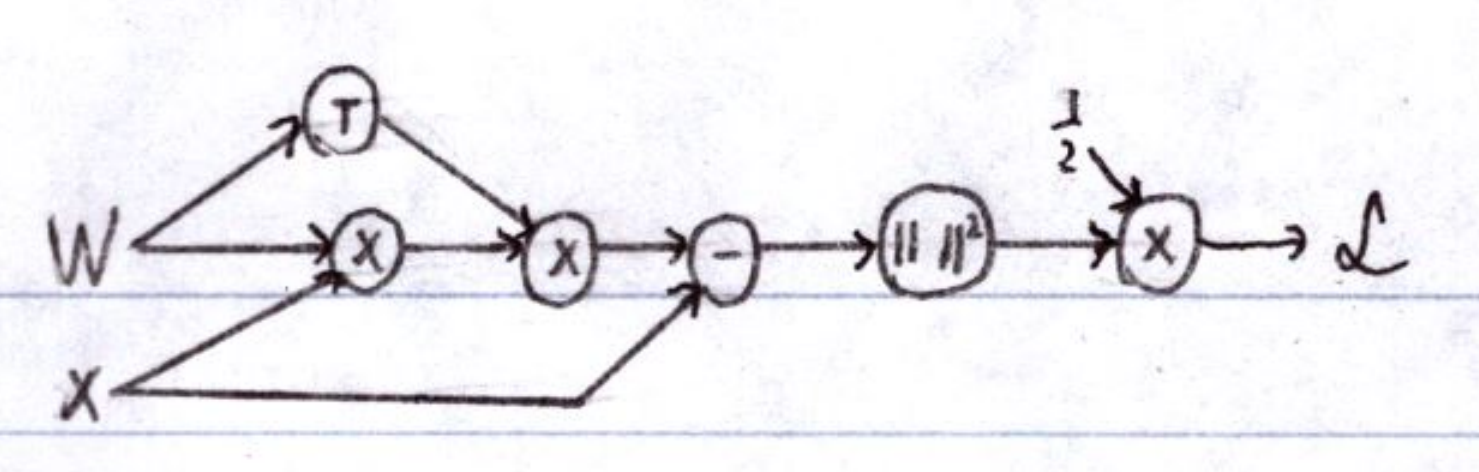
\includegraphics[width=8cm]{img/hw3/autoencoder}
          \end{center}

    \item When there's multiple paths leading out of a node,
          to backpropagate we simply take the sum of the two gradients.

    \item I'll use the following intermediate variables:
          \begin{align*}
              \loss=\frac{e}{2}  &  & e=\norm{d}^2 \in \real &  & d=p-x \in \real^n \\
              p=W^Tr \in \real^n &  & r=Wx \in \real^m
          \end{align*}
          We can then calculate them like so:
          \begin{gather*}
              \frac{\partial \loss}{\partial e}=\frac{1}{2} \\
              \frac{\partial \loss}{\partial d}=\frac{\partial e}{\partial d} \cdot \frac{\partial \loss}{\partial e}=2d \cdot \frac{1}{2}=d \\
              \frac{\partial \loss}{\partial p}=\frac{\partial d}{\partial p} \cdot \frac{\partial \loss}{\partial d}=I \cdot d=d \\
              \frac{\partial \loss}{\partial W_1}=\left(\frac{\partial \loss}{\partial p} \cdot r^T\right)^T=rd^T \\
              \frac{\partial \loss}{\partial r}=\frac{\partial p}{\partial r} \cdot \frac{\partial \loss}{\partial p}=Wd \\
              \frac{\partial \loss}{\partial W_2}=\frac{\partial \loss}{\partial r} \cdot x^T=Wdx^T
          \end{gather*}
          To get the final gradient, we use that $\nabla_W \loss = \frac{\partial \loss}{\partial W_1}+\frac{\partial \loss}{\partial W_2}$:
          \begin{align*}
              \frac{\partial \loss}{\partial W_1}+\frac{\partial \loss}{\partial W_2}
               & = Wxd^T+Wdx^T                                             \\
               & = \boxed{Wx\left(W^TWx-x\right)+W\left(W^TWx-x\right)x^T}
          \end{align*}
\end{enumerate}

\pagebreak

\section{Backprop for Gaussian-process Latent Variable Model}

\begin{enumerate}[label=(\alph*)]
    \item Only $\beta^{-1}$ is used, so I've included it directly.
          \begin{center}
              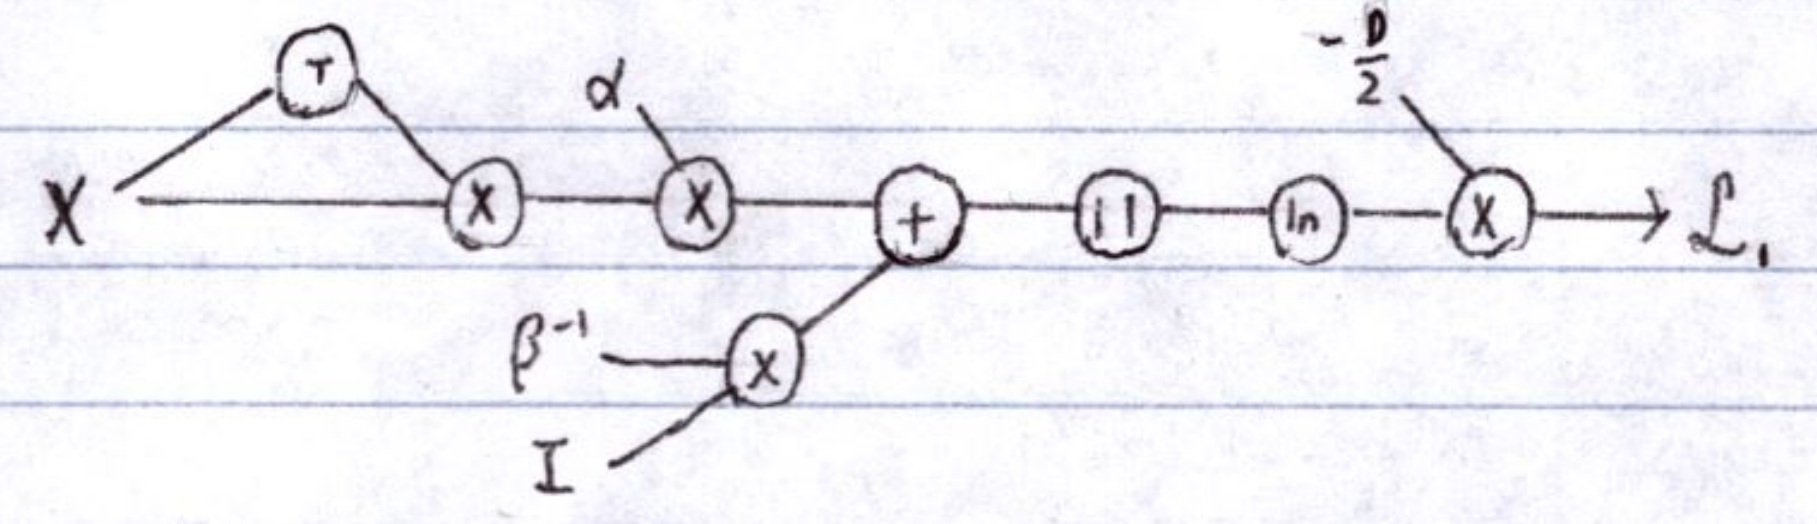
\includegraphics[width=10cm]{img/hw3/l1}
          \end{center} \label{prob:l1}

    \item Here's the intermediate variables I'm gonna use:
          \begin{align*}
              \loss_1=-\frac{D}{2} l \in \real       &  & l=\ln d \in \real                 &  & d=|K| \in \real               \\
              K=A+\beta^{-1}I \in \real^{n \times n} &  & A=\alpha B \in \real^{n \times n} &  & B=XX^T \in \real^{n \times n}
          \end{align*}
          We can then compute the gradients as follows:
          \begin{gather*}
              \frac{\partial \loss_1}{\partial l}=-\frac{D}{2} \\
              \frac{\partial \loss_1}{\partial d}=\frac{\partial l}{\partial d} \cdot \frac{\partial \loss_1}{\partial l}=-\frac{D}{2d} \\
              \frac{\partial \loss_1}{\partial K}=\frac{\partial d}{\partial K} \cdot \frac{\partial \loss_1}{\partial d}=-\frac{D|K|}{2d} \cdot \left(X^{-1}\right)^T=-\frac{D}{2}\cdot \left(X^{-1}\right)^T \\
              \frac{\partial \loss_1}{\partial A}=\frac{\partial K}{\partial A} \cdot \frac{\partial \loss_1}{\partial K}=\frac{\partial \loss_1}{\partial K} \\
              \frac{\partial \loss_1}{\partial B}=\frac{\partial A}{\partial B} \cdot \frac{\partial \loss_1}{\partial A}=\alpha \cdot \frac{\partial \loss_1}{\partial K} \\
              \frac{\partial \loss_1}{\partial X_1}=\frac{\partial \loss_1}{\partial B} \cdot \left(X^T\right)^T \\
              \frac{\partial \loss_1}{\partial X_2}=\left(X^T\frac{\partial \loss_1}{\partial B}\right)^T=\frac{\partial \loss_1}{\partial B}^T X
          \end{gather*}
          Adding the last two partial derivatives gives us
          \begin{align*}
              \frac{\partial \loss_1}{\partial X}
               & = \left(\frac{\partial \loss_1}{\partial B}+\frac{\partial \loss_1}{\partial B}^T\right) X \\
               & = \left(-\frac{D\alpha}{2}\left(X^{-1}\right)^T-\frac{D\alpha}{2}X^{-1}\right)X            \\
               & = \boxed{-\frac{D\alpha}{2}\left(X^{-T}+X^{-1}\right)X}
          \end{align*}

    \item Since $K$ was already used in $\loss_1$, I've just included it as an input here for brevity.
          We can just tack on the first part of the computation graph in \ref{prob:l1}.
          \begin{center}
              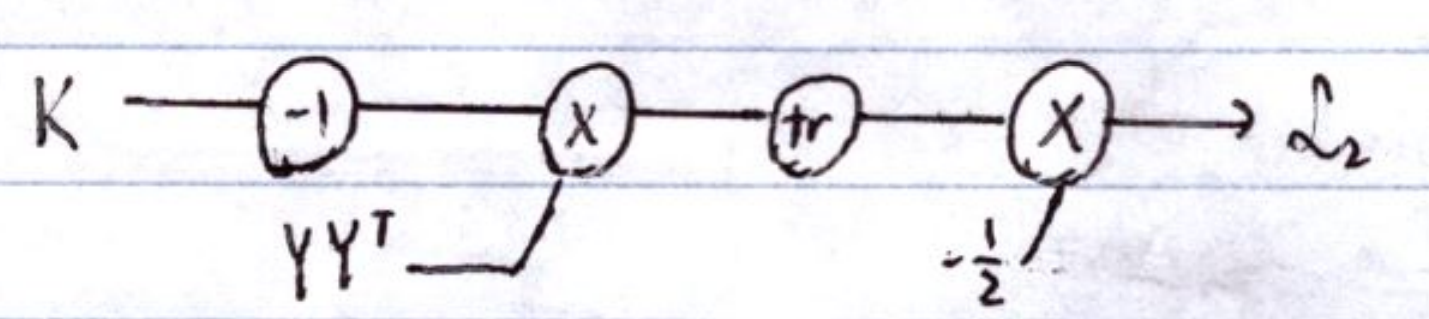
\includegraphics[width=10cm]{img/hw3/l2}
          \end{center}

    \item Here's the intermediate variables:
          \begin{align*}
              \loss_2=-\frac{1}{2}\Tr M &  & M=HYY^T \in \real^{n \times n} &  & H=K^{-1} \in \real^{n \times n}
          \end{align*}
          and then everything past $K$ is the same as in \ref{prob:l1}.
          \begin{gather*}
              \frac{\partial \loss_2}{\partial M}=-\frac{1}{2}I \\
              \frac{\partial \loss_2}{\partial H}=\frac{\partial M}{\partial H}\frac{\partial \loss_2}{\partial M}=\frac{\partial \loss_2}{\partial M}\left(YY^T\right)^T=-\frac{1}{2}YY^T \\
              \frac{\partial \loss_2}{\partial K}=-K^{-T} \frac{\partial \loss_2}{\partial H} K^{-T}
          \end{gather*}
          Now with $\frac{\partial \loss_2}{\partial K}$, we can reuse
          this computation from \ref{prob:l1}:
          \[\frac{\partial \loss_2}{\partial B}=\frac{\partial A}{\partial B} \cdot \frac{\partial \loss_2}{\partial A}=\alpha \cdot \frac{\partial \loss_2}{\partial K}\]
          which then combining with another previous result gives us
          \begin{align*}
              \frac{\partial \loss_2}{\partial X}
               & = \left(\frac{\partial \loss_2}{\partial B}+\frac{\partial \loss_2}{\partial B}^T\right) X                                    \\
               & = \alpha \left(-K^{-T} \frac{\partial \loss_2}{\partial H}K^{-T}- K^{-1} \frac{\partial \loss_2}{\partial H}^T K^{-1}\right)X \\
               & = \boxed{\frac{\alpha}{2} \left(K^{-T}YY^TK^{-T}+K^{-1}YY^TK^{-1}\right)X }
          \end{align*}

    \item We just add the two like so:
          \[\frac{\partial \loss_1}{\partial X}+\frac{\partial \loss_2}{\partial X}=
              \boxed{-\frac{D\alpha}{2}\left(X^{-T}+X^{-1}\right)X+\frac{\alpha}{2} \left(K^{-T}YY^TK^{-T}+K^{-1}YY^TK^{-1}\right)X }\]
\end{enumerate}

\pagebreak

\section{NNDL to the Rescue!}

Before we start, let's just take the derivative of the swish function:
\begin{align*}
    \frac{d \swish(k)}{dk}
     & = k \cdot \frac{d \sigma(k)}{dk} + \sigma(k) \\
     & = k\sigma(k)(1-\sigma(k))+\sigma(k)          \\
     & = \sigma(k)(\sigma(k)+k-k\sigma(k))
\end{align*}

\begin{enumerate}[label=(\alph*)]
    \item "SM" stands for the softmax function.
          \begin{center}
              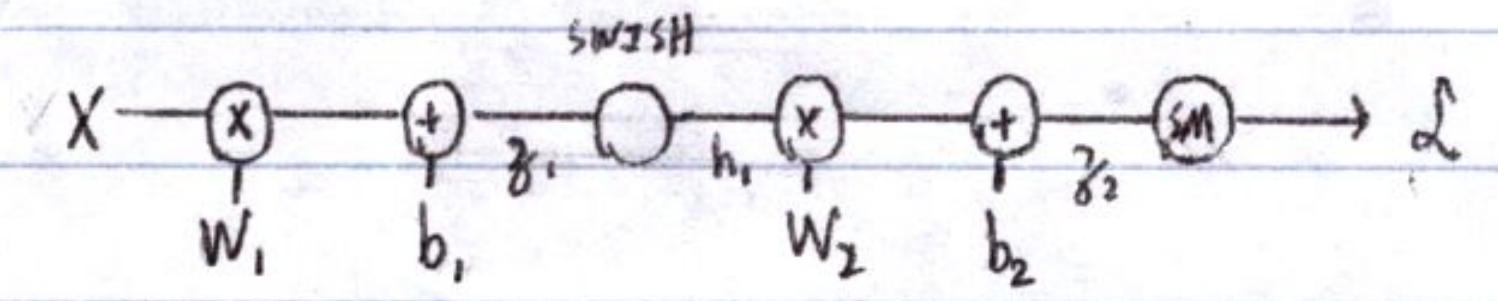
\includegraphics[width=10cm]{img/hw3/swish}
          \end{center}

    \item Note that $b_2 \in \real^C$ and $W_2 \in \real^{C \times H}$.
          \begin{align*}
              \nabla_{b_2} \loss
               & = \frac{\partial z_2}{\partial b_2} \cdot \frac{\partial \loss}{\partial z_2} \\
               & = I \cdot \frac{\partial \loss}{\partial z_2}                                 \\
               & = \boxed{\frac{\partial \loss}{\partial z_2}}
          \end{align*}
          For $W_2$ we use the tensor trick taught in class:
          \[\nabla_{W_2} \loss
              = \frac{\partial z_2}{\partial W_2} \frac{\partial \loss}{\partial z_2} \\
              = \boxed{\frac{\partial \loss}{\partial z_2} h_1^T}\]

    \item One past the second layer is $h_1$:
          \begin{gather*}
              \frac{\partial \loss}{\partial h_1}
              = \frac{\partial z_2}{\partial h_1} \cdot \frac{\partial \loss}{\partial z_2}
              = W_2^T \frac{\partial \loss}{\partial z_2}
          \end{gather*}
          and we use this to calculate the gradient wrt $z_1$:
          \begin{align*}
              \frac{\partial \loss}{\partial z_1}
               & = \frac{\partial h_1}{\partial z_1} \odot \frac{\partial \loss}{\partial h_1}                                                   \\
               & =\boxed{\sigma(z_1) \odot (\sigma(z_1)+z_1-z_1 \odot \sigma(z_1)) \odot \left(W_2^T \frac{\partial \loss}{\partial z_2}\right)}
          \end{align*}
          For brevity, we'll denote the gradients in terms of $\frac{\partial \loss}{\partial z_1}$
          which was just calculated above.
          Notice that past that it's just another linear layer, so
          \begin{gather*}
              \nabla_{b_1} \loss = \boxed{\frac{\partial \loss}{\partial z_1}} \\
              \nabla_{W_1} \loss = \boxed{\frac{\partial \loss}{\partial z_1}x^T} \\
          \end{gather*}
\end{enumerate}

\end{document}
